%!TEX TS-program = xelatex
\documentclass{article}
\usepackage[utf8]{inputenc}
\usepackage{dirtree}
\usepackage{listings}
\usepackage{color}
\usepackage{fancyhdr}
\usepackage{amsmath}
\usepackage{graphicx}
\usepackage{csvsimple}
\usepackage{url}
\usepackage{hyperref}
\usepackage{booktabs}
\usepackage{tabularx}
\usepackage[margin=0.8in]{geometry}
\usepackage{float}
\usepackage{subfig}
\usepackage{listings}
\usepackage{upgreek}
\usepackage[american]{circuitikz}
\usepackage[titletoc,title]{appendix}
\usepackage{amssymb}
\usepackage{array,etoolbox}
\usepackage[parfill]{parskip}
\usepackage{ragged2e}
\usepackage{pgfplots}
\usepackage{pdfpages}
\usepackage{svg}
\usepackage{lastpage}
\usepackage{xcolor}
\hypersetup{
    colorlinks,
    linkcolor={red!50!black},
    citecolor={blue!50!black},
    urlcolor={blue!80!black}
}
\pgfplotsset{width=10cm,compat=1.9} 
\usepgfplotslibrary{external}
\tikzexternalize 

\preto\tabular{\setcounter{magicrownumbers}{0}}
\newcounter{magicrownumbers}
\newcommand\rownumber{\stepcounter{magicrownumbers}\arabic{magicrownumbers}}
\newcommand{\ruler}{\noindent\rule{\textwidth}{1pt}}

% Standard colors for the code syntax highlighting.
\definecolor{pblue}{rgb}{0.13,0.13,1}
\definecolor{pgreen}{rgb}{0,0.5,0}
\definecolor{pred}{rgb}{0.9,0,0}
\definecolor{pgrey}{rgb}{0.46,0.45,0.48}

\def\doubleunderline#1{\underline{\underline{#1}}}
\newcommand{\doubleindent}{\indent \indent}

% Define Y colymntype
\newcolumntype{Y}{>{\centering\arraybackslash}X}

% Header for each page (except first)
\pagestyle{fancy}
\fancyhf{}
\fancyhead[LE,RO]{\authors}
\fancyhead[RE,LO]{\coursecode}
\fancyfoot[L,RO]{\thepage}

\definecolor{mygreen}{rgb}{0,0.6,0}
\definecolor{mygray}{rgb}{0.5,0.5,0.5}
\definecolor{mymauve}{rgb}{0.58,0,0.82}

\lstset{ 
  backgroundcolor=\color{white},   % choose the background color; you must add \usepackage{color} or \usepackage{xcolor}; should come as last argument
  basicstyle=\footnotesize,        % the size of the fonts that are used for the code
  breakatwhitespace=false,         % sets if automatic breaks should only happen at whitespace
  breaklines=true,                 % sets automatic line breaking
  captionpos=b,                    % sets the caption-position to bottom
  commentstyle=\color{mygreen},    % comment style
  deletekeywords={...},            % if you want to delete keywords from the given language
  escapeinside={\%*}{*)},          % if you want to add LaTeX within your code
  extendedchars=true,              % lets you use non-ASCII characters; for 8-bits encodings only, does not work with UTF-8
  frame=single,	                   % adds a frame around the code
  keepspaces=true,                 % keeps spaces in text, useful for keeping indentation of code (possibly needs columns=flexible)
  keywordstyle=\color{blue},       % keyword style
  language=C,                      % the language of the code
  numbers=left,                    % where to put the line-numbers; possible values are (none, left, right)
  numbersep=5pt,                   % how far the line-numbers are from the code
  numberstyle=\tiny\color{mygray}, % the style that is used for the line-numbers
  rulecolor=\color{black},         % if not set, the frame-color may be changed on line-breaks within not-black text (e.g. comments (green here))
  showspaces=false,                % show spaces everywhere adding particular underscores; it overrides 'showstringspaces'
  showstringspaces=false,          % underline spaces within strings only
  showtabs=false,                  % show tabs within strings adding particular underscores
  stepnumber=1,                    % the step between two line-numbers. If it's 1, each line will be numbered
  stringstyle=\color{mymauve},     % string literal style
  tabsize=4,	                   % sets default tabsize to 2 spaces
  title=\lstname                   % show the filename of files included with \lstinputlisting; also try caption instead of title
}

% Group name
\newcommand{\groupname}{Group}

% Define author information
\newcommand{\authors}{Philip Hjortsberg, William Wennerström}
\newcommand{\authorsinfo}{
    \underline{\groupname{}:} \\ \\
    Philip Hjortsberg* \thanks{*E-post: \texttt{phihjo-2@student.ltu.se}} \\
    William Wennerström$\dagger$ \thanks{$\dagger$E-post: \texttt{wenwil-5@student.ltu.se}}
}

% Define course information
\newcommand{\coursename}{Design of Dynamic Web Systems}
\newcommand{\coursecode}{M7011E}

% Define project name
\newcommand{\projectname}{Project Roaster}

% Define information about the school/university
\newcommand{\schoolinfo}{Department of Computer Science, \\
                         Electrical and Space Engineering \\
                         \bigskip{}
                         Luleå University of Technology \\
                         Luleå, Sweden
}

\title{
    \coursecode{} \\
    \coursename{} \\
    \vspace{1.8em}
    \textbf{\projectname{}} \break
    \author{
        \authorsinfo{}
    } \break{}
    \schoolinfo{}}
\renewcommand\footnotemark{}
    \date{\today}
 
\pagestyle{fancy}
\fancyhf{}
 
\rfoot{Page \thepage \hspace{1pt} of \pageref{LastPage}}
 
\begin{document}

\maketitle
\newpage

{\hypersetup{linkcolor=black}
    \tableofcontents}
\newpage

\section{The problem}
One of the big pains when programming in groups is code that is unreadable. Many times you can look at a code snippet and see who wrote that piece
just based on the formatting and comments. The solution to this is to enforce a uniform code and documentation style that every person adheres to.
This is normally done by installing a linting tool chain and configuring it equally on all systems used for developing. 
The idea for this project is to eliminate the installing and configuring step by doing it all in the site called Roaster, along with the intriguing feature of following your own and friends code quality progress.

Roast analyzes and grades your code. The user can register and follow their personal programming progress and compare it with people you follow! 
You could compare it to music scrobbling, but for code.
Personal statistics is generated by running static code analysis on the uploaded code - data such as number of errors, number of warnings and even code style problems is collected.
The statistics can then be viewed in a feed where both your own and your friends progress is listed.
Global statistics like most common errors and number of rows analyzed is displayed on a page that can be viewed by everyone.

\section{System design}

\section{System architecture}
The system architecture is designed to be deploy able independently of underlying platform. This led us to containerize the server in order to facilitate the deployment process and avoid installation mishaps. Both the databases are not containerized as there is no gain in doing so.
The whole architecture is intended to be scalable as implemented right now in Amazon Web Services (AWS). If the solution is to be deployed at some other hosting solution like your own servers, and scalability is wanted, one would need to implement an load balancer in front of all the application servers. It's also wise to setup a heavily tested reverse proxy on the load balancer, like nginx and setup the TLS certificates here. To match the size of your application server you would maybe like to scale the databases. Since these to not run in docker or with any special configurations, it should be easy to just follow standard best practices for clustering Redis and PostgreSQL.
The communication between the application server and the databases are not encrypted as of now since they are all hosted in a Virtual Private Cloud (VPC) in AWS and thereby sandboxed. If implementing this on your own data centre or hardware you have to decide on this your self in order to secure the architecture. The application server has support for encrypted communication between both databases. 

The front end is based on a JavaScript framework called Mithril.js that encourages modularization and a model component based pattern. This takes advantage of a virtual DOM that utilizes diffing which makes it very fast, and mitigates many security risks like XSS attacks. 

\begin{figure}[H]
  \centering
  \includesvg[width=14cm]{architecture.svg}
  \caption{System architecture overview.}
\end{figure}
\section{Application Programming Interface}
\section{Technology choices}
\section{Description of software parts and interaction between them}

\newpage

\section{Security considerations}
Several security issues has been taken into consideration when developing the system.

\subsection{HTTPS/TLS}
The connection from the client to the web server is made over TLS with a Amazon signed certificate.
This is configured by the Elastic Load Balancer running on Elastic Beanstalk that acts like a reverse proxy.
The request then propagates through our VPC (Virtual Private Cloud) in AWS in plaintext. 

\subsection{CSRF}
\label{subsec:csrf}
The site has implemented protection against CSRF (Cross Site Request Forgery). CSRF is a man-in-the-middle attack where the automatic cookie submission (the cookie is always sent for every request by the web browser) is abused. A site that utilizes cross-origin requests cannot use the \texttt{site-only} attribute for cookies, i.e. another malicious website open in another tab can also issue authenticated requests to the web service\cite{rick}.

In order to increase the security against CSRF attacks we have chosen to use and implement a rolling random token scheme. The rolling scheme will ensure that the CSRF token is not stolen as demonstrated by the BREACH attack\cite{breach}. First, a CSRF cookie is issued by the web server to sign challenges against, then a challenge is issued by the web server as a HTTP header called \texttt{X-CSRF-Token} for every request.

We also had to implement our own network handling when using XHR requests in the frontend due to the CSRF mitigation system. The library we have implemented, called \texttt{Network}\cite{roaster-network}, wraps the Mithril.js \texttt{m.request} method and retrieves the new \texttt{X-CSRF-Token} header for every requests and then saves it so it can be used for the next XHR request.

All HTTP methods, except \texttt{GET, HEAD, OPTIONS} and \texttt{TRACE}, that are sent to the web server are required to authenticate with the CSRF challenge response mechanism. Therefore the \texttt{Network} library creates a \texttt{HEAD} request toward the \texttt{/} (root) API endpoint to receive the first initial \texttt{X-CSRF-Token} for the rolling scheme.

\subsection{XSS}
The Mithril.js framework will automatically escape all HTML tag characters before inserting into the Virtual DOM that it creates\cite{mithril-trust}. Therefore most XSS (Cross Site Scripting) issues are mitigated. However, because we also use jQuery which \textit{does not} escape HTML tag characters, the escaping is done explicitly for the search bar component. Removing the jQuery dependency is discussed in the \hyperref[subsec:remove-jquery]{Future work - Remove jQuery} section below.

\subsection{Secure cookies}
Our user session cookies is stored in the cookie store in the browser. These are validated with the HMAC verification mechanism and encrypted with AES-256. HMAC verification ensures that the cookie content has not been tampered with during the transfer\cite{fips-198}. While AES-256 encrypts the data contained within the cookie, ensuring that no one can read it\cite{fips-197}. Even with TLS these are real issues due to the BREACH/CRIME vulnerability that is able to extract the HTTP headers for encrypted transfers\cite{breach}. The BREACH attack is mitigated using the rolling CSRF token scheme explained above in \hyperref[subsec:csrf]{Security considerations - CSRF}

\subsection{Password storage}
There are a lot of challenges keeping user credentials secured. Our solution is based on well known algorithms, Bcrypt and SHA-512. The implementation uses official libraries in Go, the language in which the server is written, so that we don't make the mistake of "rolling our own crypto".

The plaintext password that is provided by the user will first be transformed to a hash sum with SHA-512. This is due to that Bcrypt limits the input to 72 bytes. By hashing the password with SHA-512 more entropy of the original password is kept. Also, some implementations of Bcrypt that allows for longer passwords can be vulnerable to DoS attacks\cite{bcrypt-length}.

The SHA-512 hash sum is then hashed again using Bcrypt. This is because
SHA-512 is a \textit{fast} hash algorithm not made for password hashing. Bcrypt is
designed to be slow and hard to speed up using hardware such as FPGAs and
ASICs. The work factor is set to 12 which should make the expensive Blowfish
setup take $> 250$ ms ($364.815906$ ms precisely on one of our laptops).
The Bcrypt algorithm also takes care of salting of the password and prepends 
it with the resulting hash.

Dropbox has a great article\cite{dropbox-passwords} on their password hashing scheme which our
scheme shares many similarities with, we do not, however, use AES-256 with a
global pepper (shared global encryption key) which is overkill for our use
case. They also encode their SHA-512 with base 64, which is not needed in our
case because we can save the hash as raw bytes (PostgreSQL's \texttt{bytea}).

Some implementations of Bcrypt uses a null byte (\texttt{\textbackslash{}x00}) to determine the end
of the input\cite{bcrypt-bug}, the Go implementations does \textit{not} have this problem. So there
is no need to encode the data as base 64. This is verified using the program
we have created in the \texttt{cmd/testbcrypt} source folder.

The approach used by Dropbox where they encode with base $64$ will generate a
$\approx 88$ byte long key, which is then truncated to $72$ bytes. This results in a
input with $64^{72}$ possible combinations. Our approach of not encoding the
input as base $64$ results in a $64$ byte long key (the output size of SHA-512),
where there is 256 possible combinations \textit{per byte}. This results in a input
with $256^{64}$ possible combinations. Therefore our approach allows for far more
possible entropy because $64^{72} \ll 256^{64}$ ($\approx 1,2 \times 10^{24}$ times more!).

\section{References to material}


\section{Discussion}
\section{Future work}
\label{sec:future-work}

\subsection{Remove jQuery}
\label{subsec:remove-jquery}
jQuery is used for the search feature and was added due to time constraints, in the future the search component can be implemented with Mithril.js and the jQuery dependency can be removed, thus removing the overhead of having to mitigate XSS injections for non-Mithril.js components.
 
 \newpage
\apptocmd{\sloppy}{\hbadness 10000\relax}{}{} 
{\RaggedRight\begin{thebibliography}{1}

\bibitem{rick}
Ramgattie, R (2018, May 14) {\em  Cracking Java’s RNG for CSRF - Javax Faces and Why CSRF Token Randomness Matters.}
Fetched 2019-01-10, from:
\url{https://blog.securityevaluators.com/cracking-javas-rng-for-csrf-ea9cacd231d2}.

\bibitem{breach}
Gluck, Y., Harris N., \& Prado A. (2013, July 12) {\em BREACH: Reviving the Crime Attack, pp. 3, 11} \\
Fetched 2019-01-10, from:
\url{http://breachattack.com/resources/BREACH%20-%20SSL,%20gone%20in%2030%20seconds.pdf}

\bibitem{roaster-network}
LuleaUniversityOfTechnology/2018-project-roaster (2019) {\em 2018-project-roaster/network.ts at 19529..28560.}
Fetched 2019-01-10, from:
\url{https://github.com/LuleaUniversityOfTechnology/2018-project-roaster/blob/1952964/www/src/services/network.ts#L38}.

\bibitem{mithril-trust}
Mithril.js 2.0.0-rc3 (2018) {\em trust(html) - Mithril.js}
Fetched 2019-01-10, from:
\url{https://mithril.js.org/trust.html#how-it-works}

\bibitem{fips-198}
NIST (2002, March 2) {\em FIPS 198-1, The Keyed-Hash Message Authentication Code (HMAC), p. 1} \\
Fetched 2019-01-10, from:
\url{https://ia902804.us.archive.org/2/items/DTIC_ADA401868/DTIC_ADA401868.pdf}

\bibitem{fips-197}
NIST (2001, November 26) {\em FIPS 197, Annoucing the Advanced Encryption Standard (AES), p. 5} \\
Fetched 2019-01-10, from:
\url{https://ia802809.us.archive.org/0/items/DTIC_ADA403903/DTIC_ADA403903.pdf}

\bibitem{bcrypt-length}
Goodin, D (2013, September 16) {\em Long passwords are good, but too much length can be a DoS hazard} \\
Fetched 2019-01-10, from:
\url{https://arstechnica.com/information-technology/2013/09/long-passwords-are-good-but-too-much-length-can-be-bad-for-security/}

\bibitem{dropbox-passwords}
Akhawe, D. (2016, September 21) {\em How Dropbox securely stores your passwords} \\
Fetched 2019-01-10, from:
\url{https://blogs.dropbox.com/tech/2016/09/how-dropbox-securely-stores-your-passwords/}

\bibitem{bcrypt-bug}
Ferrara, A (2015, March 12) {\em Security Issue: Combining Bcrypt With Other Hash Functions} \\
Fetched 2019-01-10, from:
\url{https://blog.ircmaxell.com/2015/03/security-issue-combining-bcrypt-with.html}

\end{thebibliography}}

\appendix
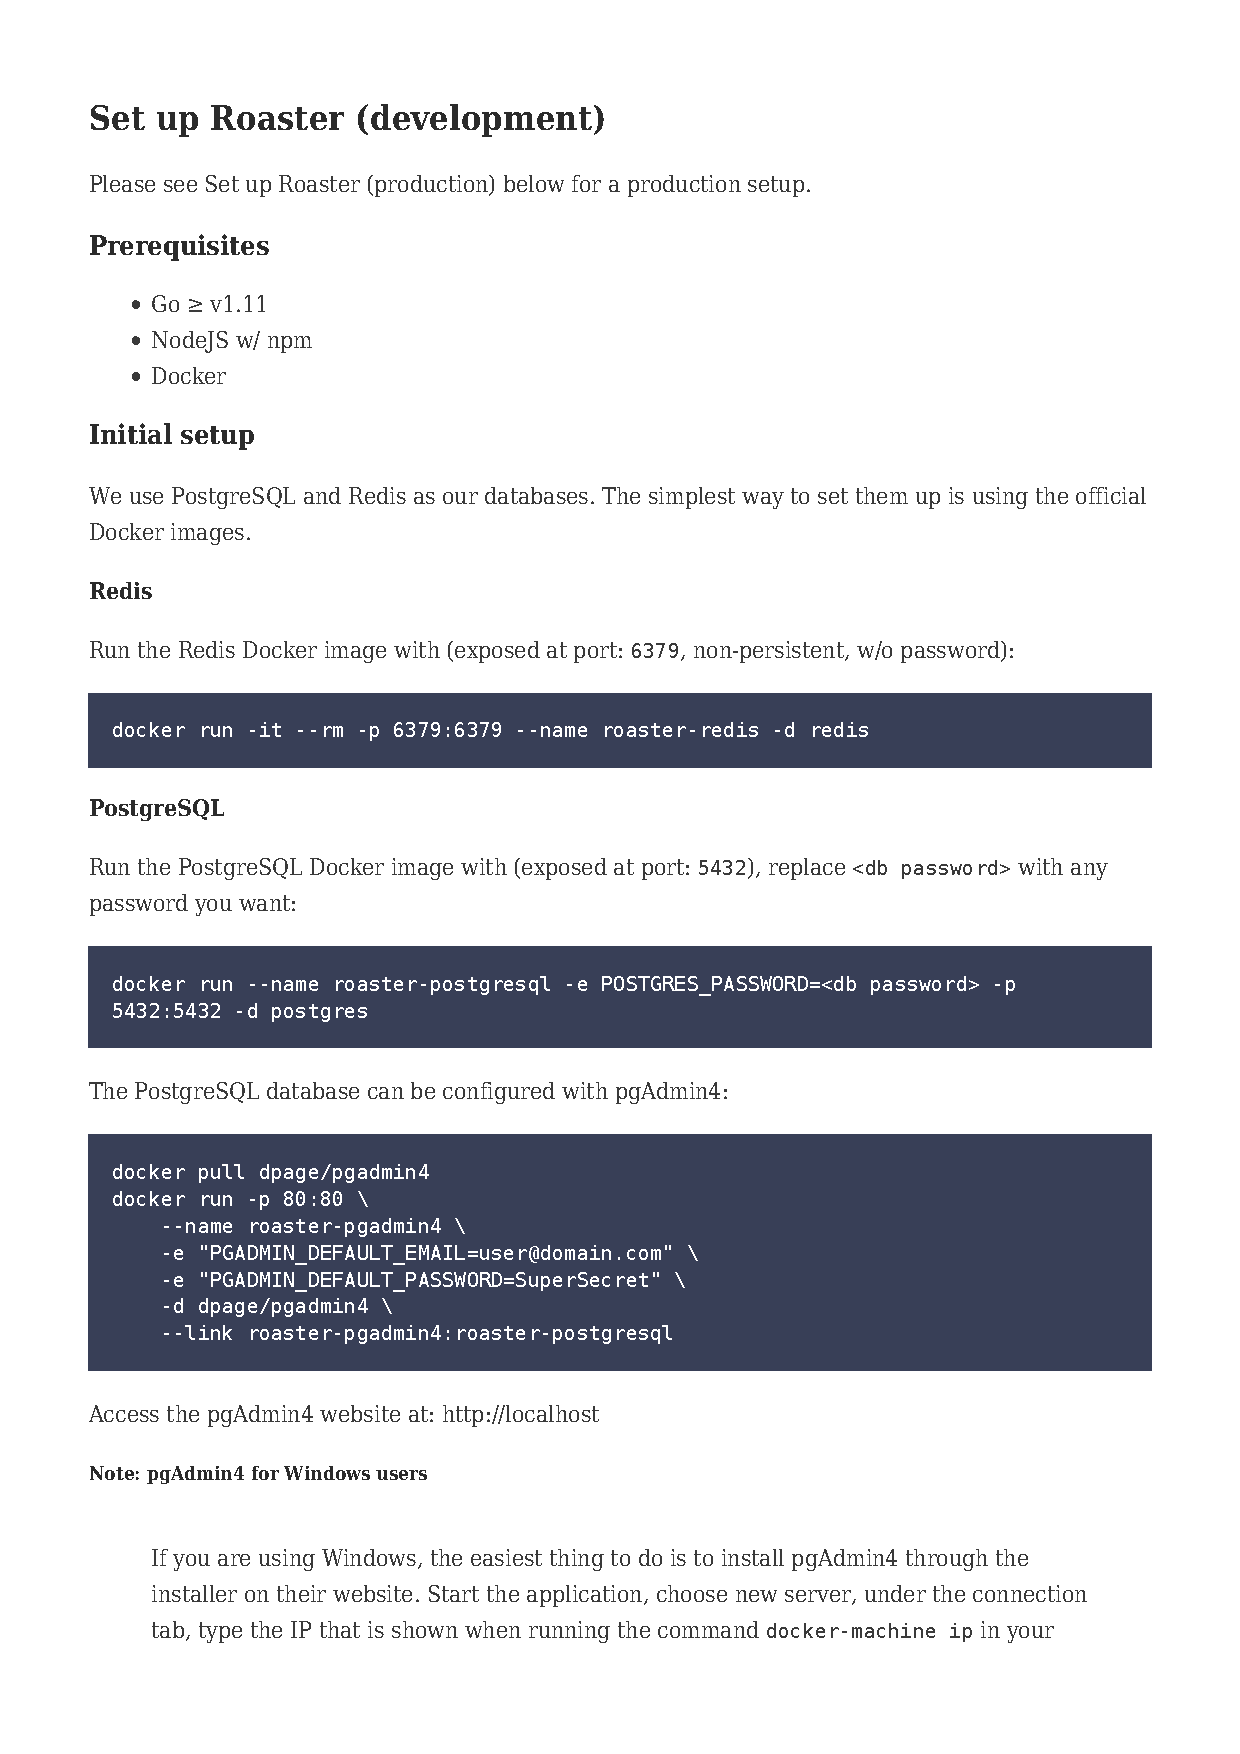
\includepdf[page=-]{install.pdf}

% Here follows some good to have examples.
\if false

\begin{figure}[H]
    \centering
    \includegraphics[width=6cm]{xxx.png}
    \caption{Lalalala.}
    \label{fig:my_label}
\end{figure}

\begin{verbatim}
PaymentTest > entitledFullAmount[ID: 505] FAILED
    java.lang.AssertionError: expected:<4960> but was:<5960>
        at org.junit.Assert.fail(Assert.java:88)
        at org.junit.Assert.failNotEquals(Assert.java:834)
        at org.junit.Assert.assertEquals(Assert.java:645)
        at org.junit.Assert.assertEquals(Assert.java:631)
        at PaymentTest.entitledFullAmount(PaymentTest.java:164)
\end{verbatim}

\begin{table}[H]
\centering
\caption{API endpoints and their methods}
\begin{tabular}{|clcl|}
\hline
\textbf{Method}              & \textbf{Endpoint}                             & \textbf{Access}              & \textbf{Description}                 \\ \hline
\multicolumn{1}{|c|}{GET}    & \multicolumn{1}{l|}{/}                        & \multicolumn{1}{c|}{N/A}     & Home page                            \\
\multicolumn{1}{|c|}{GET}    & \multicolumn{1}{l|}{/login}                   & \multicolumn{1}{c|}{N/A}     & View customer login page                      \\
\multicolumn{1}{|c|}{POST}   & \multicolumn{1}{l|}{/login}                   & \multicolumn{1}{c|}{N/A}     & Login customer user                           \\
\multicolumn{1}{|c|}{GET}    & \multicolumn{1}{l|}{/register}                & \multicolumn{1}{c|}{N/A}     & View customer register page                   \\
\multicolumn{1}{|c|}{POST}   & \multicolumn{1}{l|}{/register}                & \multicolumn{1}{c|}{N/A}     & Register customer user                        \\
\multicolumn{1}{|c|}{GET}    & \multicolumn{1}{l|}{/user}                    & \multicolumn{1}{c|}{C, W, A} & View user page                       \\
\multicolumn{1}{|c|}{POST}   & \multicolumn{1}{l|}{/user}                    & \multicolumn{1}{c|}{C, W, A} & Set user information                 \\
\multicolumn{1}{|c|}{GET}    & \multicolumn{1}{l|}{/article?id=\{0..n\}}     & \multicolumn{1}{c|}{C, W, A} & Get specific article by ID           \\
\multicolumn{1}{|c|}{POST}   & \multicolumn{1}{l|}{/cart}                    & \multicolumn{1}{c|}{C}       & Add artice to cart                   \\
\multicolumn{1}{|l|}{DELETE} & \multicolumn{1}{l|}{/cart?pos=\{0..n\}}       & \multicolumn{1}{c|}{C}       & Delete article from cart by position \\
\multicolumn{1}{|l|}{DELETE} & \multicolumn{1}{l|}{/cart}                    & \multicolumn{1}{c|}{C}       & Delete whole cart                    \\
\multicolumn{1}{|c|}{GET}    & \multicolumn{1}{l|}{/cart}                    & \multicolumn{1}{c|}{C}       & View cart                            \\
\multicolumn{1}{|c|}{PUT}    & \multicolumn{1}{l|}{/cart}                    & \multicolumn{1}{c|}{C}       & Order items in cart                  \\
\multicolumn{1}{|c|}{GET}    & \multicolumn{1}{l|}{/order}                   & \multicolumn{1}{c|}{W, A}    & View current orders                  \\
\multicolumn{1}{|c|}{GET}    & \multicolumn{1}{l|}{/order?id=\{0..n\}}       & \multicolumn{1}{c|}{W, A}    & View order by ID                     \\
\multicolumn{1}{|c|}{GET}    & \multicolumn{1}{l|}{/warehouse}               & \multicolumn{1}{c|}{W}       & Warehouse user home page             \\
\multicolumn{1}{|c|}{GET}    & \multicolumn{1}{l|}{/admin}                   & \multicolumn{1}{c|}{A}       & Admin user home page                 \\
\multicolumn{1}{|c|}{PUT}    & \multicolumn{1}{l|}{/order?id=\{0..n\}}       & \multicolumn{1}{c|}{W}       & Accept order by ID                   \\
\multicolumn{1}{|c|}{GET}    & \multicolumn{1}{l|}{/user?id=\{0..n\}}        & \multicolumn{1}{c|}{A}       & Display user by ID                   \\
\multicolumn{1}{|c|}{GET}    & \multicolumn{1}{l|}{/search?query=\{string\}}        & \multicolumn{1}{c|}{N/A}       & Search for article                   \\
\multicolumn{1}{|c|}{POST}   & \multicolumn{1}{l|}{/register?type=admin}     & \multicolumn{1}{c|}{A}       & Register new admin user              \\
\multicolumn{1}{|c|}{POST}   & \multicolumn{1}{l|}{/register?type=warehouse} & \multicolumn{1}{c|}{A}       & Register new warehouse user          \\
\multicolumn{1}{|c|}{POST}   & \multicolumn{1}{l|}{/register?type=customer}  & \multicolumn{1}{c|}{A}       & Register new customer user           \\ \hline
\end{tabular}
\end{table}
\fi
\end{document}
